\documentclass[11pt,openany]{article}

\usepackage{mathtools, commath}
% Packages for formatting
\usepackage[margin=1in]{geometry}
\usepackage{fancyhdr}
\usepackage{enumerate}
\usepackage{graphicx}
\usepackage{kotex}
\usepackage{arydshln} % Include this package
\usepackage{bbding}
\usepackage{amsmath}
\usepackage{amsthm}
\usepackage[dvipsnames,table]{xcolor}
\usepackage{amssymb, amsfonts}
\usepackage{wasysym}
\usepackage{footnote}
\usepackage{tablefootnote}
\usepackage{arydshln} % Include this package
% Fonts
\usepackage[T1]{fontenc}
\usepackage[utf8]{inputenc}
\usepackage{newpxtext,newpxmath}
\usepackage{sectsty}

% Define colors
\definecolor{TealBlue1}{HTML}{0077c2}
\definecolor{TealBlue2}{HTML}{00a5e6}
\definecolor{TealBlue3}{HTML}{b3e0ff}
\definecolor{TealBlue4}{HTML}{00293c}
\definecolor{TealBlue5}{HTML}{e6f7ff}

\definecolor{thmcolor}{RGB}{231, 76, 60}
\definecolor{defcolor}{RGB}{52, 152, 219}
\definecolor{lemcolor}{RGB}{155, 89, 182}
\definecolor{corcolor}{RGB}{46, 204, 113}
\definecolor{procolor}{RGB}{241, 196, 15}

\usepackage{color,soul}
\usepackage{soul}
\newcommand{\mathcolorbox}[2]{\colorbox{#1}{$\displaystyle #2$}}
\usepackage{cancel}
\newcommand\crossout[3][black]{\renewcommand\CancelColor{\color{#1}}\cancelto{#2}{#3}}
\newcommand\ncrossout[2][black]{\renewcommand\CancelColor{\color{#1}}\cancel{#2}}

\usepackage{hyperref}
\usepackage{booktabs}

% Chapter formatting
\definecolor{titleTealBlue}{RGB}{0,53,128}
\usepackage{titlesec}
\titleformat{\section}
{\normalfont\sffamily\Large\bfseries\color{titleTealBlue!100!gray}}{\thesection}{1em}{}
\titleformat{\subsection}
{\normalfont\sffamily\large\bfseries\color{titleTealBlue!50!gray}}{\thesubsection}{1em}{}

%Tcolorbox
\usepackage[most]{tcolorbox}
\usepackage{multirow}
\usepackage{multicol}

\usepackage[linesnumbered,ruled]{algorithm2e}
\usepackage{algpseudocode}
\usepackage{setspace}
\SetKwComment{Comment}{/* }{ */}
\SetKwProg{Fn}{Function}{:}{end}
\SetKw{End}{end}
\SetKw{DownTo}{downto}

% Define a new environment for algorithms without line numbers
\newenvironment{algorithm2}[1][]{
	% Save the current state of the algorithm counter
	\newcounter{tempCounter}
	\setcounter{tempCounter}{\value{algocf}}
	% redefine the algorithm numbering (remove prefix)
	\renewcommand{\thealgocf}{}
	\begin{algorithm}
	}{
	\end{algorithm}
	% Restore the algorithm counter state
	\setcounter{algocf}{\value{tempCounter}}
}

\usepackage{adjustbox}
% Header and footer formatting
\pagestyle{fancy}
\fancyhead{}
\fancyhf{}
\rhead{\textcolor{TealBlue2}{\large\textbf{기대수(기초부터 대학원 수학까지 시리즈) 3기}}}%\rule{3cm}{0.4pt}}
\lhead{\textcolor{TealBlue2}{\large\textbf{수학의 즐거움, Enjoying Math}}}
% Define footer
%\newcommand{\footer}[1]{
%\begin{flushright}
%	\vspace{2em}
%	\includegraphics[width=2.5cm]{school_logo.jpg} \\
%	\vspace{1em}
%	\textcolor{TealBlue2}{\small\textbf{#1}}
%\end{flushright}
%}
%\rfoot{\large Department of Information Security, Cryptogrphy and Mathematics, Kookmin Uni.\includegraphics[height=1.5cm]{school_logo.jpg}}
\fancyfoot{}
\fancyfoot[C]{-\thepage-}

\usepackage{tcolorbox}
\tcbset{colback=white, arc=5pt}

\definecolor{axiomcolor}{HTML}{a88bfa}
\definecolor{defcolor}{RGB}{52, 152, 219}
\definecolor{procolor}{RGB}{241, 196, 15}
\definecolor{thmcolor}{RGB}{231, 76, 60}
\definecolor{lemcolor}{RGB}{155, 89, 182}
\definecolor{corcolor}{RGB}{46, 204, 113}
\definecolor{execolor}{RGB}{90, 128, 127}

% Define a new command for the custom tcolorbox
\newcommand{\axiombox}[2][]{%
	\begin{tcolorbox}[colframe=axiomcolor, title={\color{white}\bfseries #1}]
		#2
	\end{tcolorbox}
}

\newcommand{\defbox}[2][]{%
	\begin{tcolorbox}[colframe=defcolor, title={\color{white}\bfseries #1}]
		#2
	\end{tcolorbox}
}

\newcommand{\lembox}[2][]{%
	\begin{tcolorbox}[colframe=lemcolor, title={\color{white}\bfseries #1}]
		#2
	\end{tcolorbox}
}

\newcommand{\probox}[2][]{%
	\begin{tcolorbox}[colframe=procolor, title={\color{white}\bfseries #1}]
		#2
	\end{tcolorbox}
}

\newcommand{\thmbox}[2][]{%
	\begin{tcolorbox}[colframe=thmcolor, title={\color{white}\bfseries #1}]
		#2
	\end{tcolorbox}
}

\newcommand{\corbox}[2][]{%
	\begin{tcolorbox}[colframe=corcolor, title={\color{white}\bfseries #1}]
		#2
	\end{tcolorbox}
}



\usepackage{amsthm}

% Define custom theorem styles
\newtheoremstyle{dotless} % Name of the style
{3pt} % Space above
{3pt} % Space below
{\itshape} % Body font
{} % Indent amount
{\bfseries} % Theorem head font
{} % Punctuation after theorem head
{2.5mm} % Space after theorem head
{} % Theorem head spec

\newtheoremstyle{definitionstyle} % Name of the style
{3pt} % Space above
{3pt} % Space below
{} % Body font
{} % Indent amount
{\bfseries} % Theorem head font
{.} % Punctuation after theorem head
{2.5mm} % Space after theorem head
{} % Theorem head spec

% Applying custom styles
\theoremstyle{dotless}
\newtheorem{theorem}{Theorem} % Theorem environment with section-wise numbering
\newtheorem{proposition}[theorem]{Proposition} % Theorem environment with section-wise numbering
\newtheorem{lemma}[theorem]{Lemma} % Lemma shares the counter with theorem
\newtheorem{corollary}[theorem]{Corollary} % Corollary shares the counter with theorem

\theoremstyle{definitionstyle}
\newtheorem*{observation}{\textcolor{Magenta}{Observation}}
\newtheorem{definition}{Definition} % Definition shares the counter with theorem
\newtheorem{example}{Example} % Example shares the counter with theorem
\newtheorem{exercise}{Exercise} % Example shares the counter with theorem
\newtheorem{remark}{Remark} % Remark shares the counter with theorem
\newtheorem*{note}{Note}

\newtheorem*{definition*}{Definition} % Definition shares the counter with theorem
\newtheorem*{example*}{Example} % Example shares the counter with theorem
\newtheorem*{exercise*}{\textcolor{violet}{Exercise}} % Example shares the counter with theorem
\newtheorem*{remark*}{Remark} % Remark shares the counter with theorem


\usepackage{tikz}
\usepackage{tikz-cd}
\usepackage{tikz-3dplot}
\usepackage{pgfplots}
\pgfplotsset{compat=newest} % Adjust to your version of pgfplots
\def\Circlearrowleft{\ensuremath{%
		\rotatebox[origin=c]{180}{$\circlearrowleft$}}}
\def\Circlearrowright{\ensuremath{%
		\rotatebox[origin=c]{180}{$\circlearrowright$}}}
\def\CircleArrowleft{\ensuremath{%
		\reflectbox{\rotatebox[origin=c]{180}{$\circlearrowleft$}}}}
\def\CircleArrowright{\ensuremath{%
		\reflectbox{\rotatebox[origin=c]{180}{$\circlearrowright$}}}}
\usetikzlibrary{
	3d, % For 3D drawing
	angles,
	arrows,
	arrows.meta,
	backgrounds,
	bending,
	calc,
	decorations.pathmorphing,
	decorations.pathreplacing,
	decorations.markings,
	fit,
	matrix,
	patterns,
	patterns.meta,
	positioning,
	quotes,
	shadows,
	shapes,
	shapes.geometric,
	tikzmark
}
\tikzset{
	% single mid‐path arrow
	mid arrow/.style={
		decoration={
			markings,
			mark=at position 0.5 with {\arrow{Stealth[scale=1.2]}}
		},
		postaction={decorate},
	},
	% style for field arrows
	field arrow/.style={
		-{Stealth[scale=1.0]},
		thick,
		blue!70!black,
	},
}
\newcommand{\ie}{\textnormal{i.e.}}
\newcommand{\rsa}{\mathsf{RSA}}
\newcommand{\rsacrt}{\mathsf{RSA}\textendash\mathsf{CRT}}
\newcommand{\inv}[1]{#1^{-1}}

%New Command
%\newcommand{\set}[1]{\left\{#1\right\}}
\newcommand{\N}{\mathbb{N}}
\newcommand{\Z}{\mathbb{Z}}
\newcommand{\Q}{\mathbb{Q}}
\newcommand{\R}{\mathbb{R}}
\newcommand{\cR}{\mathcal{R}}
\newcommand{\C}{\mathbb{C}}
\newcommand{\F}{\mathbb{F}}
\newcommand{\nbhd}{\mathcal{N}}
\newcommand{\Log}{\operatorname{Log}}
\newcommand{\Arg}{\operatorname{Arg}}
\newcommand{\pv}{\operatorname{P.V.}}

\newcommand{\of}[1]{\left( #1 \right)} 
%\newcommand{\abs}[1]{\left\lvert #1 \right\rvert}
%\newcommand{\norm}[1]{\left\| #1 \right\|}

\newcommand{\sol}{\textcolor{magenta}{\bf Sol}}
\newcommand{\conjugate}[1]{\overline{#1}}

\newcommand{\res}{\operatorname{res}}
\DeclareMathOperator*{\Res}{\operatorname{Res}}

%\renewcommand{\Re}{\operatorname{Re}}
%\renewcommand{\Im}{\operatorname{Im}}

\newcommand{\cyclic}[1]{\langle #1 \rangle}
\newcommand{\uniform}{\overset{\$}{\leftarrow}}
\newcommand{\xmark}{\textcolor{red}{\XSolidBrush}}
\newcommand{\vmark}{\textcolor{green!75!black}{\CheckmarkBold}}

\newcommand{\gen}[1]{\langle #1 \rangle}
\newcommand{\Gen}[1]{\left\langle #1 \right\rangle}

\newcommand{\img}[1]{\text{Img}(#1)}
\newcommand{\Img}[1]{\text{Img}\left(#1\right)}
\newcommand{\preimg}[1]{\text{Img}^{-1}(#1)}
\newcommand{\Preimg}[1]{\text{Img}^{-1}\left(#1\right)}

\newcommand{\relation}{\mathrel{\mathcal{R}}}
\newcommand{\injection}{\rightarrowtail}
\newcommand{\surjection}{\twoheadrightarrow}
\newcommand{\id}{\textnormal{id}}

\newcommand{\eqclass}[1]{\left[#1\right]}

% Define custom colors for O and X
\newcommand{\yes}{\textcolor{blue}{\bf \fullmoon}}
\newcommand{\no}{\textcolor{red}{\bf \texttimes}}

\DeclarePairedDelimiter\ceil{\lceil}{\rceil}
\DeclarePairedDelimiter\floor{\lfloor}{\rfloor}
%\renewcommand{\floor}[#1]{\lfloor #1\rfloor}
%\newcommand{\Floor}[#1]{\left\lfloor #1\right\rfloor}
%\newcommand{\ceil}[#1]{\lceil #1\rceil}
%\newcommand{\Ceil}[#1]{\left\lceil #1\right\rceil}

\newcommand{\topology}{\mathscr{T}}
\newcommand{\sequence}[1]{\langle #1\rangle}

\setstretch{1.25}
\begin{document}
\pagenumbering{arabic}
\begin{center}
	\huge\textbf{Topology I}\\
	\vspace{0.5em}
	\large{Ji, Yong-hyeon}\\
	\vspace{0.5em}
	\normalsize{\today}\\
\end{center}

\noindent 
We cover the following topics in this note.
\begin{itemize}
	\item Topology; Topological Space
	\item Open Set
	\item Continuous Mapping
	\item \st{Distance Function; Metric Topology}
\end{itemize}
\hrule\vspace{12pt}
%Preliminaries:
%\begin{itemize}
%	\item Boundedness, Supremum and Infimum
%	\item Least Upper Bound Property (Completeness Axiom)
%	\item Well-Ordering Principle and Mathematical Induction
%	\item Archimedean Property
%\end{itemize}
%\hrule\vspace{12pt}
\begin{center}
\begin{minipage}{.32\textwidth}\centering
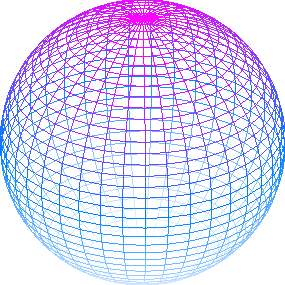
\includegraphics[scale=.8]{../tikz/grad-math-tikz-pdf/sphere.pdf}
\end{minipage}\hfill
\begin{minipage}{.32\textwidth}\centering
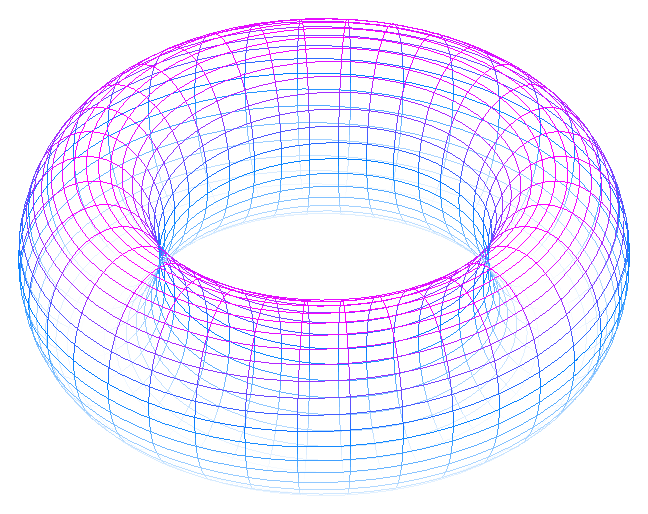
\includegraphics[scale=.45]{../tikz/grad-math-tikz-pdf/torus.pdf}
\end{minipage}\hfill
\begin{minipage}{.32\textwidth}\centering
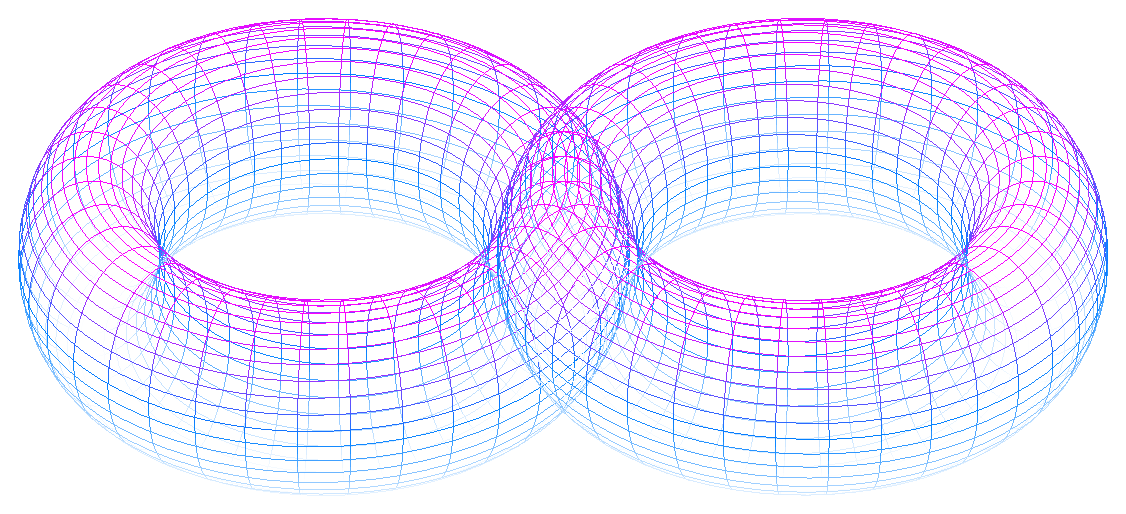
\includegraphics[scale=.3]{../tikz/grad-math-tikz-pdf/double-torus.pdf}
\end{minipage}
\end{center}
\vfill
\begin{center}
\begin{minipage}{.32\textwidth}\centering
	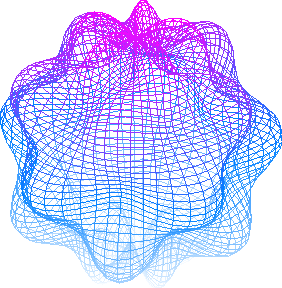
\includegraphics[scale=.8]{../tikz/grad-math-tikz-pdf/sphere2.pdf}
\end{minipage}\hfill
\begin{minipage}{.32\textwidth}\centering
	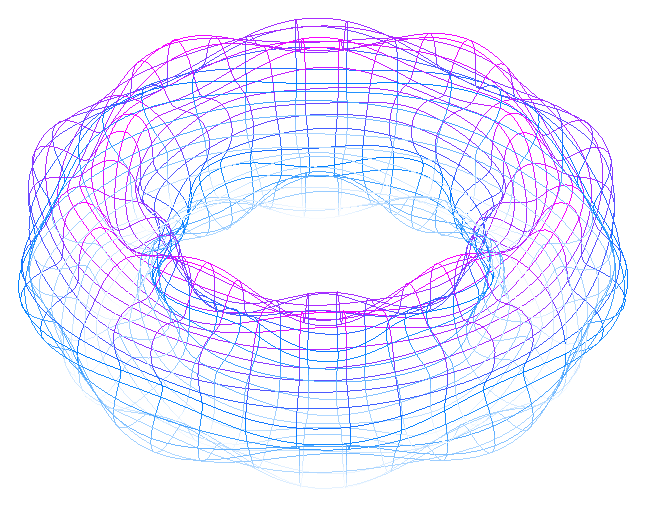
\includegraphics[scale=.45]{../tikz/grad-math-tikz-pdf/torus2.pdf}
\end{minipage}\hfill
\begin{minipage}{.32\textwidth}\centering
	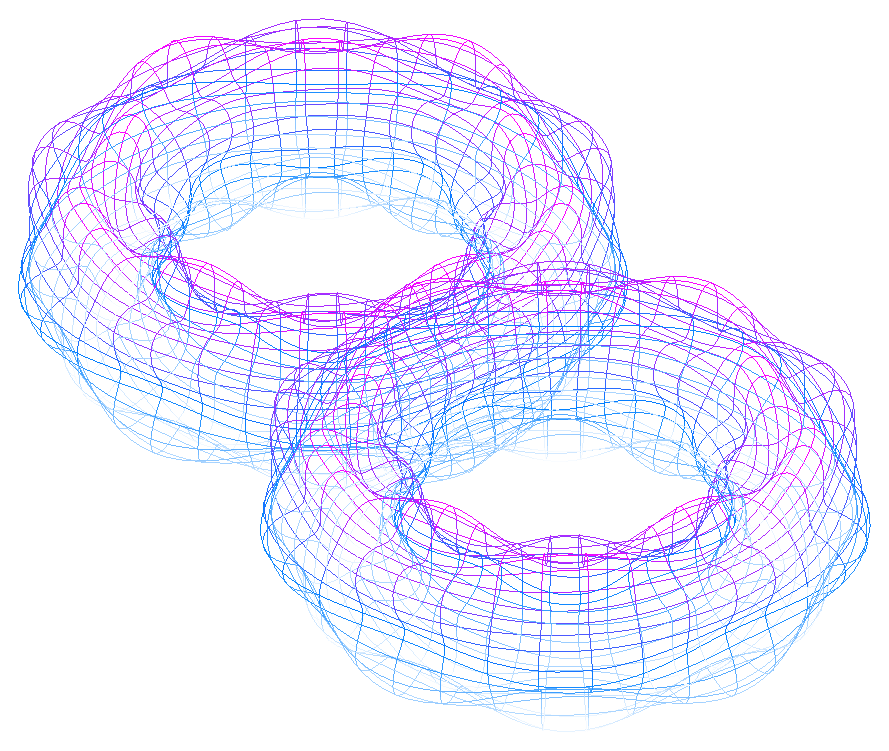
\includegraphics[scale=.35]{../tikz/grad-math-tikz-pdf/double-torus2.pdf}
\end{minipage}
\end{center}
\vfill
\begin{center}
\begin{minipage}{.32\textwidth}\centering
	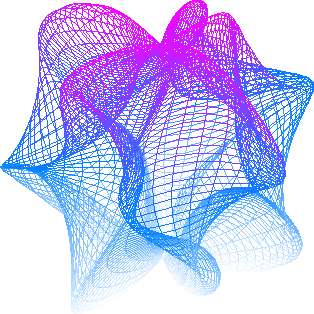
\includegraphics[scale=.8]{../tikz/grad-math-tikz-pdf/sphere3.pdf}
\end{minipage}\hfill
\begin{minipage}{.32\textwidth}\centering
	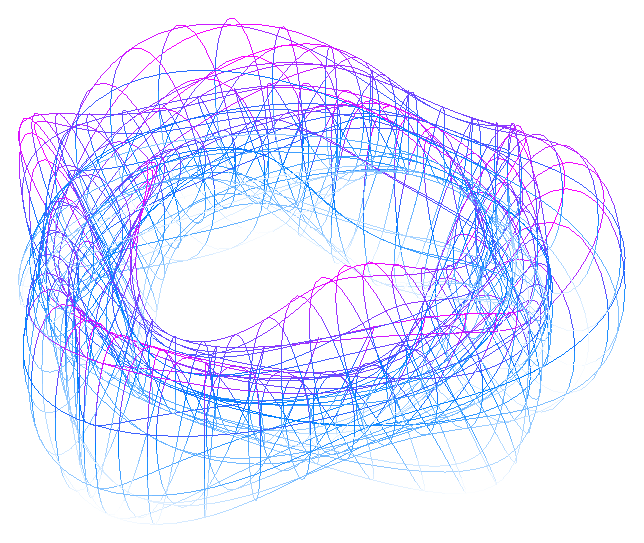
\includegraphics[scale=.45]{../tikz/grad-math-tikz-pdf/torus3.pdf}
\end{minipage}\hfill
\begin{minipage}{.32\textwidth}\centering
	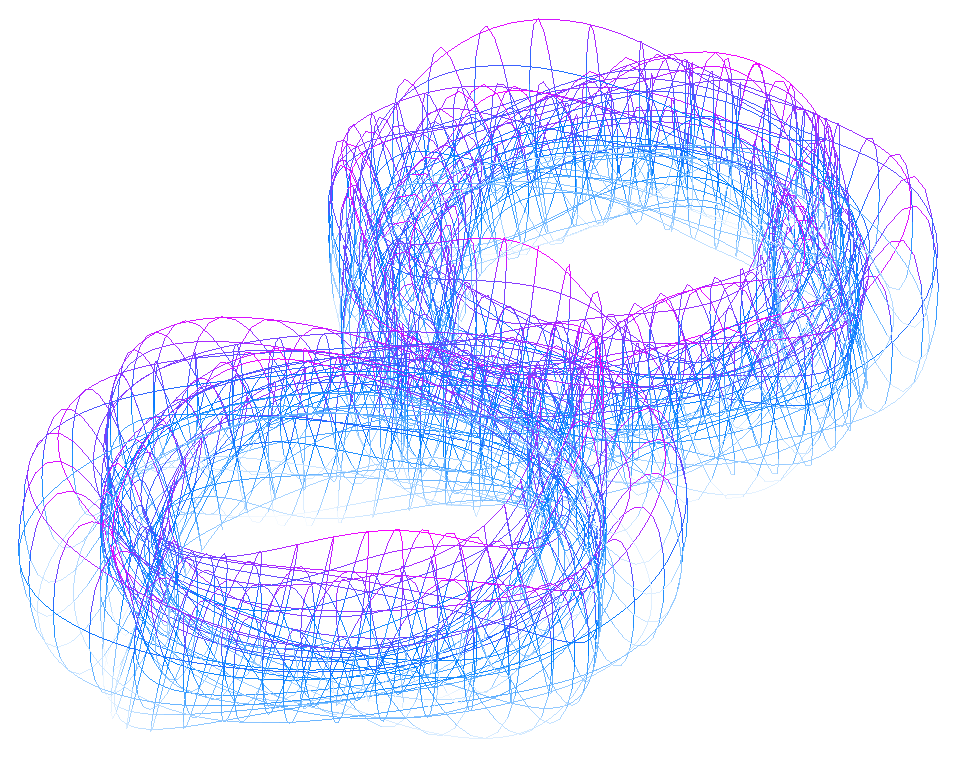
\includegraphics[scale=.35]{../tikz/grad-math-tikz-pdf/double-torus3.pdf}
\end{minipage}
\end{center}
\vfill
%\definecolor{mypurple}{HTML}{4C9FFF}
%\begin{center}
%\begin{tikzpicture}
%%	\def \x{3}
%%	\def \y{3.5}
%%	\draw[very thin,color=gray!15,step=.5] (-\x,-\y) grid (\x,\y);
%%	
%%	\foreach \i in {-\x,...,-2,-1,1,2,...,\x}
%%	\draw[gray] (\i,.1)--(\i,-.1) node[below] {$\i$};%x-axis
%%	\foreach \i in {-\y,-1,1,1,\y}
%%	\draw[gray] (.1,\i)--(-.1,\i) node[left] {$\i$};%y-axis
%	\begin{scope}[yshift=.5cm]
%	\node[mypurple] at (-4,2.75) {\LARGE\bf Length};
%	\draw[mypurple, line width=1mm] (-1,3) -- (1,3);
%	\draw[mypurple, line width=1mm] (-2,2.5) -- (2,2.5);
%	\end{scope}
%	\node[mypurple] at (-4,.5) {\LARGE\bf Area};
%	\filldraw[mypurple] (-2,0) rectangle (-1,1);
%	\filldraw[mypurple] (0,-1) rectangle (3,2);
%	\begin{scope}[yshift=-.5cm]	
%	\node[mypurple] at (-4,-2) {\LARGE\bf Angle};
%	\draw[mypurple, fill=mypurple, line width=.5mm] (-1.5,-1.5) -- (-2.5,-3) -- (-.5,-3) -- cycle;
%	\draw[mypurple, fill=mypurple, line width=.5mm] (.5,-3) -- (2.5,-3) -- (2.5, -1.5) -- cycle;
%	\end{scope}
%\end{tikzpicture}
%\end{center}
\vfill

\defbox[Topology]{\begin{definition*}
Let $S$ be a non-empty set. A \textbf{topology} on $S$ is a subset \[
\topology=\set{U:U\subseteq S}\subseteq 2^S
\] that satisfies the axioms: \begin{itemize}
	\item[(O1)] $S$ and $\varnothing$ are elements of $\topology$:\quad $S\in\topology$ and $\varnothing\in\topology$.
	\item[(O2)\footnote{$\topology$ is closed under \textit{arbitrary} unions}] The union of an arbitrary subset of $\topology$
	is an element of $\topology$: \[
	\set{U_\alpha}_{\alpha\in\Lambda}\subseteq\topology\implies\bigcup_{\alpha\in\Lambda}U_\alpha\in\topology.
	\]
	\item[(O3)\footnote{$\topology$ is closed under \textit{finite} intersection}] The intersection of any finite subset of $\topology$
	is an element of $\topology$: \[
	\set{U_i}_{i=1}^n\subseteq\topology\implies\bigcap_{i=1}^n U_i\in\topology.
	\]
\end{itemize}
\end{definition*}}
\begin{remark*}
	By mathematical induction, we have \[
	\text{O3}\iff [\set{U_1,U_2}\subseteq\topology\Rightarrow U_1\cap U_2\in\topology].
	\]
\end{remark*}

%\begin{example}
%	Consider a set $S=\set{a,b,c,d,e}$. \begin{center}
%\begin{tikzpicture}[scale=.75]
%%	\def \x{3}
%%	\def \y{3}
%%	\draw[very thin,color=gray!15,step=.5] (-\x,-\y) grid (\x,\y);
%%	
%%	\foreach \i in {-\x,...,-2,-1,1,2,...,\x}
%%	\draw[gray] (\i,.1)--(\i,-.1) node[below] {$\i$};%x-axis
%%	\foreach \i in {-\y,-1,1,1,\y}
%%	\draw[gray] (.1,\i)--(-.1,\i) node[left] {$\i$};%y-axis
%	
%	\draw[rounded corners=8pt] (0, 3) -- (-1.5, 2.5) -- (-3, 1) -- (-2, .9) -- (-1.9, 0) -- (-2.5, -1) -- (-3, -2.5) -- (-2, -2) -- (0,-3) -- (2, -1.5) -- (3,-.5) -- (3,.5) -- (2, 1) -- (1.5, 1.5) -- (1.75, 2.5) -- cycle;
%	
%	\filldraw (0,1.5) circle (2pt) node[above] {$a$};
%	\filldraw (-1,.5) circle (2pt) node[above] {$c$};
%	\filldraw (1,0) circle (2pt) node[above] {$d$};
%	\filldraw (-.5,-2) circle (2pt) node[above] {$b$};
%	\filldraw (.5,-1) circle (2pt) node[above] {$e$};
%\end{tikzpicture}
%	\end{center}
%\begin{center}
%\begin{minipage}{.32\textwidth}
%\begin{tikzpicture}[scale=.75]
%%	\def \x{3}
%%	\def \y{3}
%%	\draw[very thin,color=gray!15,step=.5] (-\x,-\y) grid (\x,\y);
%%	
%%	\foreach \i in {-\x,...,-2,-1,1,2,...,\x}
%%	\draw[gray] (\i,.1)--(\i,-.1) node[below] {$\i$};%x-axis
%%	\foreach \i in {-\y,-1,1,1,\y}
%%	\draw[gray] (.1,\i)--(-.1,\i) node[left] {$\i$};%y-axis
%	
%	\draw[rounded corners=8pt] (0, 3) -- (-1.5, 2.5) -- (-3, 1) -- (-2, .9) -- (-1.9, 0) -- (-2.5, -1) -- (-3, -2.5) -- (-2, -2) -- (0,-3) -- (2, -1.5) -- (3,-.5) -- (3,.5) -- (2, 1) -- (1.5, 1.5) -- (1.75, 2.5) -- cycle;
%	
%	\filldraw (0,1.5) circle (2pt) node[above] {$a$};
%	\filldraw (-1,.5) circle (2pt) node[above] {$c$};
%	\filldraw (.5,0) circle (2pt) node[above] {$d$};
%	\filldraw (-.5,-1.5) circle (2pt) node[above] {$b$};
%	\filldraw (1,-1.5) circle (2pt) node[above] {$e$};
%	
%	\draw[line width=.5mm, opacity=.5, magenta] (0, 1.5) circle (10pt);
%	\draw[line width=.5mm, opacity=.5, orange, rotate=-20, xshift=-.15cm, yshift=.15cm] (0,0) ellipse (1.25cm and .5cm);
%	\draw[line width=.5mm, opacity=.5, green!50!black, yshift=.5cm] (0, 0) circle (40pt);
%	\draw[line width=.5mm, opacity=.5, cyan=-20, rotate=-20, xshift=0cm, yshift=-.5cm] (0,0) ellipse (1.75cm and 1.5cm);
%\end{tikzpicture}
%\end{minipage}
%\end{center}
%\end{example}

\defbox[Topological Space]{\begin{definition*}
	Let $S$ be a set. Let $\topology$ be a topology on $S$. Then the ordered pair $(S,\topology)$ is called a \textbf{topological space}.
\end{definition*}}
\defbox[Open Set]{\begin{definition*}
	Let $(S,\topology)$ be a topological space. $E\subseteq S$ is an \textbf{open set}, or \textbf{open} (in $S$) iff $E\in\topology$.
\end{definition*}}
\begin{remark*}
A subset $\topology\subseteq 2^S$ is a topology on $S$ if and only if \begin{enumerate}
	\item[(i)] $\varnothing$ and $S$ are open;
	\item[(ii)] Let $\set{E_\alpha}_{\alpha\in\Lambda}\subseteq\topology$. Then $\displaystyle\bigcup_{\alpha\in\Lambda}E_\alpha$ is open.
	\item[(iii)] Let $\set{E_i}_{i=1}^n\subseteq\topology$. Then $\displaystyle\bigcap_{i=1}^n E_i$ is open.
\end{enumerate}
\end{remark*}
\defbox[Continuous Mapping]{\begin{definition*}
	Let $(X,\topology_X)$ and $(Y,\topology_Y)$ are topological spaces. Let $f:X\to Y$ be a mapping from $X$ to $Y$. \begin{enumerate}[(1)]
		\item (Continuous at a Point) Let $x\in X$. The mapping $f$ is \textbf{continuous at} $\boldsymbol{x}$ if and only if \[
		\forall U_Y\in\topology_Y,\ (f(x)\in U_Y\implies\exists U_X\in\topology_X\ \text{such that}\ x\in U_X\land f[U_X]\subseteq U_Y.)
		\]
		\item (Continuous on a Set) Let $S\subseteq X$. The mapping $f$ is \textbf{continuous on} $\boldsymbol{S}$ if and only if $f$ is continuous at every point $x\in S$.
		\item (Continuous Everywhere) The mapping $f$ is \textbf{continuous on} $\boldsymbol{X}$ if and only if \[
		U_Y\in\topology_Y\implies f^{-1}[U_Y]\in\topology_X,
		\] where $f^{-1}[U_Y]=\set{x\in X:f(x)\in U_Y}$ is the preimage of $U_Y$ under $f$.
		\begin{center}
		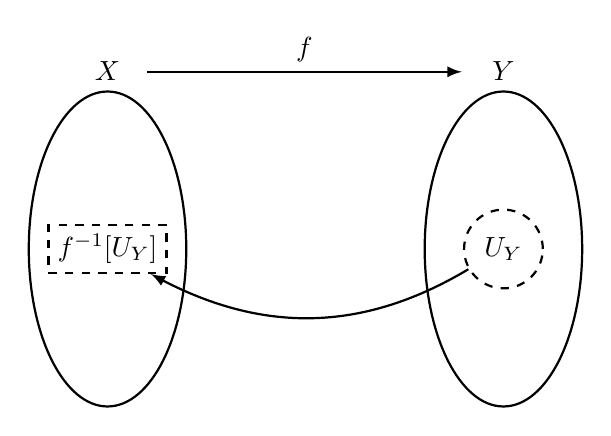
\begin{tikzpicture}[thick] 
			\node[ellipse,draw,minimum width=2cm,minimum height=4cm,label=above:$X$] (X) {};
			\node[ellipse,draw,minimum width=2cm,minimum height=4cm,right=3cm of X,label=above:$Y$]
			(Y){};
			\node[dashed,draw] (f) at (X.center) {$f^{-1}[U_Y]$};
			\node[circle,dashed,draw,minimum size=1cm] (U) at (Y.center) {$U_Y$};
			\draw[-latex] (0.5,2.25) -- (4.5,2.25) node[midway,above]{$f$};
			\draw[-latex] (U) to[bend left] (f);
		\end{tikzpicture}
		\end{center}
	\end{enumerate}
\end{definition*}}
\newpage
\lembox{\begin{lemma}
Let $X$ be a set. \begin{enumerate}[(1)]
	\item (\textbf{The Intersection of Finite Sets is Finite or Empty}) Let \( \{A_i\}_{i \in I} \) be a collection of finite sets. Then
	\[
	\bigcap_{i \in I} A_i
	\]
	is finite if \( I \) is finite, or empty otherwise.
	\item (\textbf{The Union of Finitely Many Finite Sets is Finite}) Let \( \{A_i\}_{i=1}^n \) be a finite collection of finite sets. Then
	\[
	\bigcup_{i=1}^n A_i
	\]
	is finite.
\end{enumerate}
\end{lemma}}
\newtheorem{proofpart}{Part}
\begin{proof}
	Let \( |A_i| < \infty \) for all \( i \in I \). The intersection is defined as:
	\[
	\bigcap_{i \in I} A_i = \{x \in X \mid x \in A_i \text{ for all } i \in I\}.
	\]
	
	\begin{proofpart}[Case 1: \( I \) is finite]
		Suppose \( I = \{i_1, i_2, \dots, i_n\} \) is finite. Then:
		\[
		\bigcap_{i \in I} A_i = A_{i_1} \cap A_{i_2} \cap \cdots \cap A_{i_n}.
		\]
		Since each \( A_{i_k} \) is finite, the intersection cannot introduce new elements:
		\[
		\bigcap_{k=1}^n A_{i_k} \subseteq A_{i_k} \quad \text{for all } k.
		\]
		Therefore, \( \bigcap_{i \in I} A_i \) is a subset of the smallest \( A_{i_k} \) and is finite.
		
	\end{proofpart}
	
	\begin{proofpart}[Case 2: \( I \) is infinite]
		If \( I \) is infinite, the intersection may be empty. For any \( x \in \bigcap_{i \in I} A_i \), \( x \) must belong to all \( A_i \). If the \( A_i \)'s shrink (e.g., \( A_i = \{1, 2, \dots, i\} \)), then for large \( i \), \( A_i \cap A_j = \emptyset \). Hence:
		\[
		\bigcap_{i \in I} A_i = \emptyset.
		\]
	\end{proofpart}
	
	Thus, the intersection of finite sets is finite if \( I \) is finite, or empty otherwise.
\end{proof}

\begin{proof}
	Each \( A_i \) is finite, meaning \( |A_i| < \infty \) for \( i = 1, 2, \dots, n \). The union satisfies:
	\[
	\bigcup_{i=1}^n A_i = A_1 \cup A_2 \cup \cdots \cup A_n.
	\]
	
	To compute the size of the union, we use the inclusion-exclusion principle:
	\[
	\left| \bigcup_{i=1}^n A_i \right| = \sum_{i=1}^n |A_i| - \sum_{1 \leq i < j \leq n} |A_i \cap A_j| + \cdots + (-1)^{n+1} |A_1 \cap A_2 \cap \cdots \cap A_n|.
	\]
	- Each term in this expansion represents the size of overlaps between the \( A_i \), all of which are finite because the \( A_i \)'s are finite.
	
	Since a finite sum of finite numbers is finite, we conclude that:
	\[
	\bigcup_{i=1}^n A_i
	\]
	is finite.
\end{proof}

\begin{example}[Cofinite Topology]
	Let $S$ be a set. Define a subset $\topology_C\subseteq 2^S$ by \[
	\topology_C:=\set{T\subseteq S:T^C\ \text{is a finite set}}\cup\set{\varnothing}
	\] We claim that $\topology_C$ be a topology on $S$:
	\begin{enumerate}[(i)]
		\item Clearly $\subseteq\in\topology_C$. Since $S^C=\varnothing$ and $\varnothing$ is finite, $S\in\topology$.
		\item Let $\set{E_\alpha}_{\alpha\in\Lambda}\subseteq\topology_C$. Then \[
		\of{\bigcup_{\alpha\in\Lambda} E_\alpha}^C=\bigcap_{\alpha\in\Lambda}E_\alpha^C
		\] and so
		\item 
	\end{enumerate}
\end{example}

\begin{example}[Discrete Topology]
	
\end{example}

\begin{example}[Indiscrete Topology]
	
\end{example}

\defbox[Finer and Coarser]{\begin{definition*}
	
\end{definition*}}

\newpage
\defbox[Distance Function]{\begin{definition*}
	TBA
\end{definition*}}
\defbox[Metric Topology]{\begin{definition*}
	TBA
\end{definition*}}


\vfill
\begin{thebibliography}{9}
	\bibitem{advanced_topo_a}
	수학의 즐거움, Enjoying Math. ``수학 공부, 기초부터 대학원 수학까지, 8. 위상수학 (a) 위상공간의 정의.'' YouTube Video, 41:25. Published 
	September 27, 2019. URL: \url{https://www.youtube.com/watch?v=q8BtXIFzo2Q}.
	\bibitem{advanced_topo_b}
	수학의 즐거움, Enjoying Math. ``수학 공부, 기초부터 대학원 수학까지, 9. 위상수학 (b) 해석학개론과 거리위상'' YouTube Video, 33:43. Published 
	September 29, 2019. URL: \url{https://www.youtube.com/watch?v=uJOGw7Yxk7c&t=242s}.
\end{thebibliography}
%\newpage
\appendix
\section{Complement of Family}
\begin{note}
	\[
	\left(\bigcup_{i\in\Lambda}E_i\right)^C=
	\bigcap_{i\in\Lambda}\left(E_i\right)^C
	\]
	\begin{proof}
		content...
	\end{proof}
\end{note}
\end{document}
